\section{Signal yield determination}
\label{sec:results}
In order to determine the \Bmumumu signal yield, an extended unbinned maximum-likelihood
fit is performed to the corrected mass distribution. To improve the sensitivity of the mass fit, an event-by-event uncertainty on the corrected mass is calculated by propagating the uncertainties of the PV and SV. The data is then split into two equally sized regions with high and low fractional corrected mass uncertainties. This improves the branching fraction sensitivity by approximately 11\% due to the different signal distributions in the two samples, as shown in Fig.~\ref{fig:resofit}.
\begin{figure}[t]
\centering
	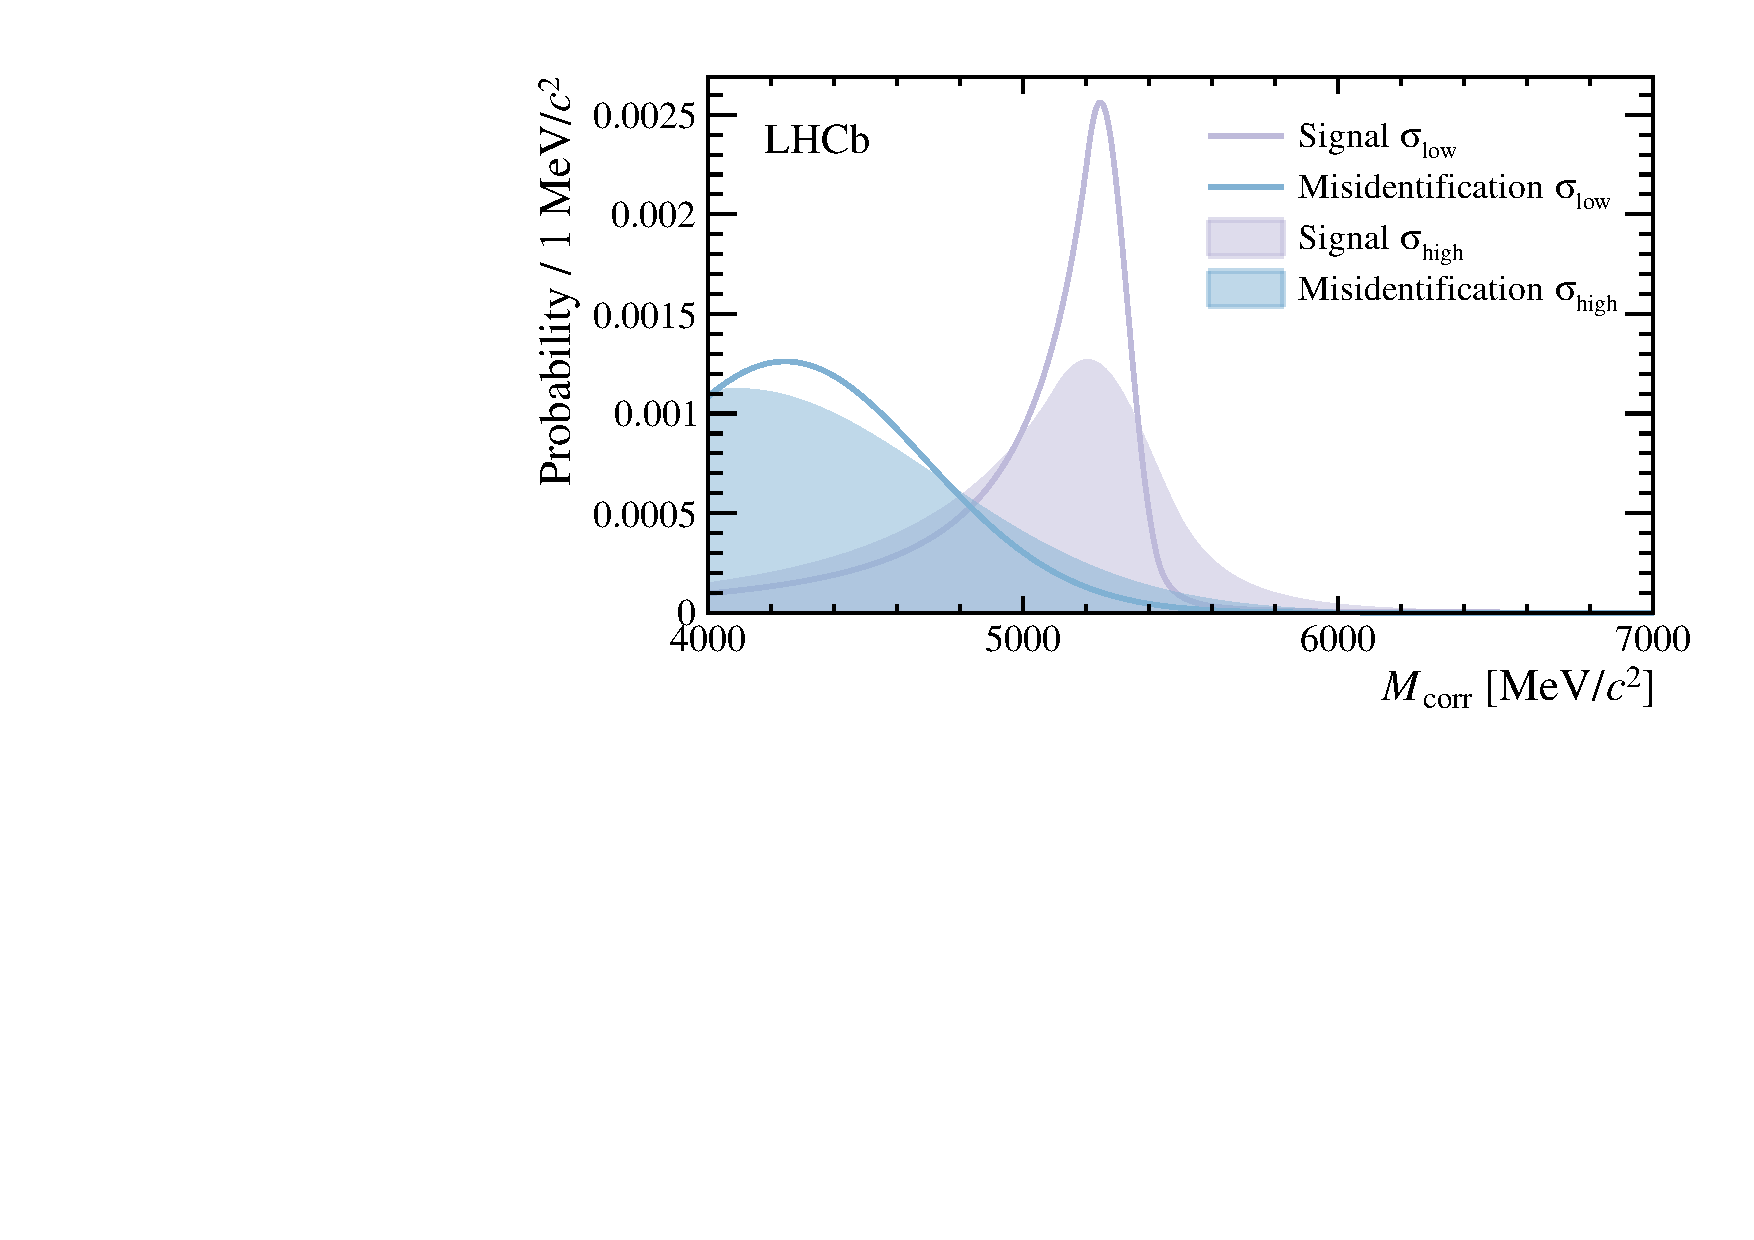
\includegraphics[width=0.85\linewidth]{Figure_3.pdf}
	\caption{\small Template distributions for signal and misidentified background
          shapes for high and low fractional corrected mass
          uncertainty. A low uncertainty on the
          corrected mass corresponds to data with better mass
          resolution. The shape of the misidentification template is
          obtained from a control sample while the signal template is
          obtained from simulation. A systematic uncertainty on the signal shape due to the choice of the signal model is not shown, as it is too small to be visible.}
\label{fig:resofit}
\end{figure}

The signal shape is modelled with the sum of two Gaussian functions with power law tails, where the tails are on both sides of the peak. The parameters of the signal shape are determined using simulation and kept fixed in the subsequent fit to the data. The combinatorial background is modelled using an exponential function, whose slope is allowed to vary in the fit and whose parameterisation is verified using simulation. The yield is left free to float in the fit.

The background from misidentified muons is obtained from the $\mumu h X$ control sample described in Sec.~\ref{sec:Misid}. The distribution and yield of this sample is fitted to a Gaussian function with a power-law tail at high corrected mass. This parameterisation is cross-checked by fitting a sample with a looser muon identification requirement. The uncertainties on the associated parameters are propagated to the fit using a multivariate Gaussian constraint. The shape and the yield of the partially reconstructed background are taken from simulation. Yields that are obtained from control samples and simulation are allowed to vary in the fit within constraints from a Poisson distribution.

\begin{figure}[t]
  \centering
  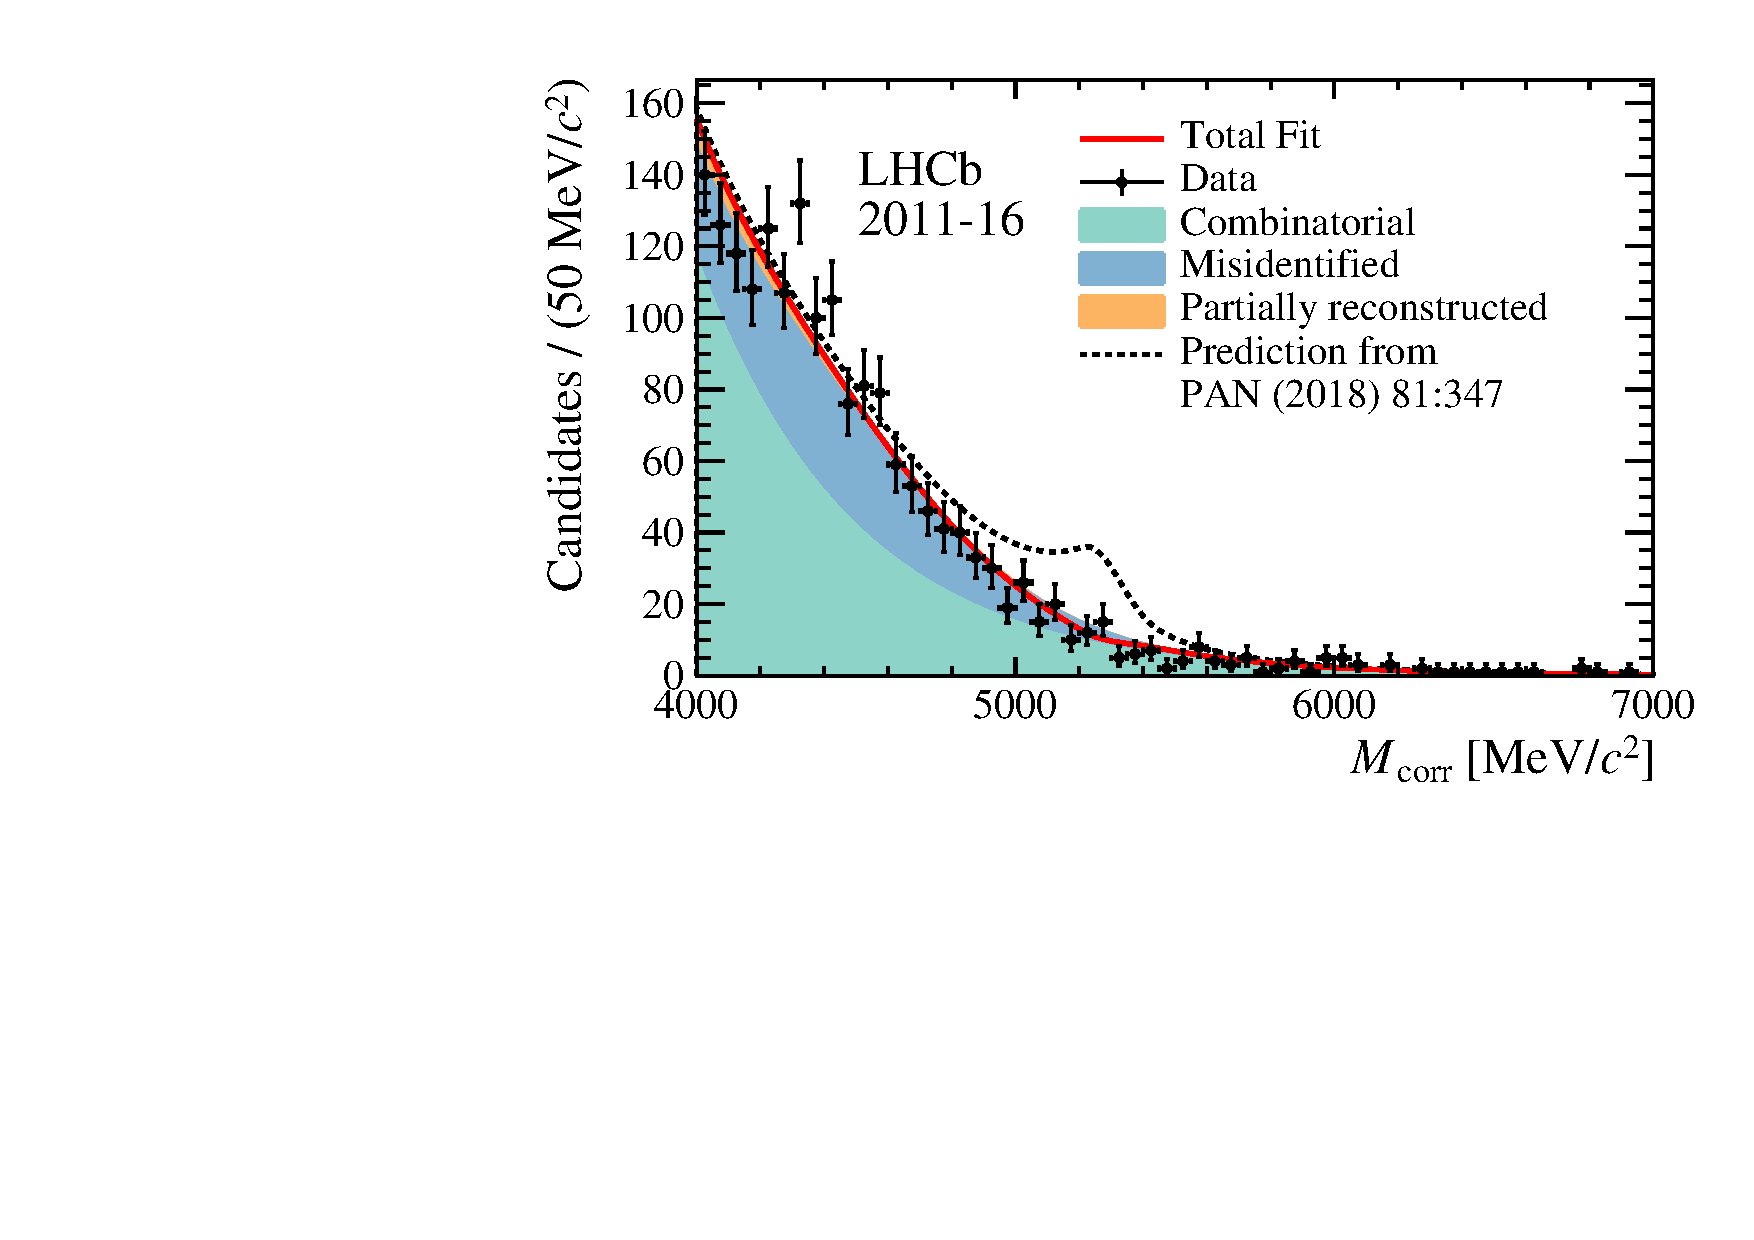
\includegraphics[width=0.85\linewidth]{Figure_4.pdf}
  \caption{\small Corrected mass distribution of the selected \Bmumumu
    candidates with the fit overlaid. Samples with low and high
    corrected mass uncertainty are fitted as individual samples but
    are merged in the figure. The fit has components for (green) combinatorial background, (blue) misidentified candidates and (orange) partially reconstructed candidates. The signal component is not visible as
    the fitted signal yield is negative. The best fit is the solid red line while the dashed line shows how the
    total would have looked like if the signal had the branching
    fraction predicted in Ref.~\cite{Danilina:2018uzr}.}
  \label{fig:signalfit}
\end{figure}
The fit to the corrected-mass distribution, combining both corrected-mass uncertainty categories, is shown in Fig.~\ref{fig:signalfit}. The signal yield is negative,  $-25\pm16$, resulting in the total fit component being slightly below the sum of the background contributions. As there is no significant signal component, a limit on the branching fraction, 
\begin{equation*}
    \BF(\decay{\Bp}{\mup\mun\mup\nu_\mu}) < 1.6\times 10^{-8}
\end{equation*}
at 95\% confidence level is set using the  $\rm{CL}_{\rm s}$ method~\cite{CLS}. 
From pseudoexperiments,
the expected upper limit is found to be $2.8\times 10^{-8}$ and the present result represents a downward
fluctuation of $1.4\sigma$. Systematic uncertainties are included in this limit and are discussed in the
following section.
